
%%% Local Variables:
%%% mode: latex
%%% TeX-master: "gis18"
%%% End:

\section{introduction}
\label{sec-intro}


\textit{Trajectory tracking} \cite{Lange:Tracking} is a combination of  two fundamental technologies of the moving objects databases (MOD), \textit{position tracking} \cite{Wolfson:PositionTracking,Leonhardi:Comparison} and \textit{trajectory simplification} \cite{Lin:Cised,Zhang:Evaluation} in one routine. In which, \textit{position tracking} is an approach that lets the MOD server effectively and efficiently know the current position of a moving object with a desired accuracy of the location information by transmitting as few messages as possible \cite{Leonhardi:Comparison}, and \textit{trajectory simplification} is to approximate the fine trajectory of the moving object with a coarse one (whose corresponding data points are a subset of the original one), such that the size of the trajectory is reduced under a constrain that the maximum distance of the former to the latter is bounded by a user specified threshold \cite{Lin:Cised,Zhang:Evaluation}. 
\textit{Position tracking} and \textit{trajectory simplification} both need to collect and send the original or reduced position information of the moving object to the MOD, meaning that redundant position information is sent to the MOD if they run separately.
%
On the other hand, if we combine them in one route as the way trajectory tracking does, then the moving object reports only one copy of its position information for both of them, such that not only the number of messages but also the size of trajectory data are reduced. 

%Position tracking and trajectory simplification share some common target and strategy, \ie reduce the number of messages or the size of trajectory data by discarding some position information that seems not that important,

Trajectory tracking is derived from position tracking whose updating protocols could be \emph{querying protocols} and \emph{reporting protocols} \cite{Leonhardi:Comparison}. Nevertheless, the most simple but efficient used updating protocol is linear dead reckoning (LDR) \cite{Leonhardi:Comparison,Civilis:Techniques,Wolfson:PositionTracking}, which is essentially an agreement between a moving object and a MOD server such that given a initial position $P_s$, a velocity $\vv{v}$ and a user specified threshold $\epsilon$, the server could infer the current position $P'$ of the object based on $P_s$ and $\vv{v}$ such that the distance from $P'$ to the actual position $P$ of the object is bounded by the threshold $\epsilon$. A moving object only updates/reports its position at the time $|P'P| \ge \epsilon$, \ie the object's locally sensed position impends to deviate from the expected one by more than the threshold \cite{Lange:Tracking}. By this way, the number of messages is reduced.
%
Though \ldr does not necessarily generate a simplified trajectory of the past movement \cite{Lange:Tracking}, the authors of \cite{Trajcevski:LDRH} find that \ldr with some small modifications is applicable to both track the positions of a moving object and simplify the trajectory built of these positions. The modified \ldr,  called \ldrh in \cite{Lange:Tracking}, is hence the first trajectory tracking algorithm that combines position tracking and trajectory simplification into one consistent process. Like \ldr, it is concise and efficient, and is suitable for resource-constraint mobile devices. However, it suffers in effectiveness in terms of compression ratio compared with other trajectory simplification algorithms \cite{Douglas:Peucker, Lin:Cised}. %, due to the nature of \ldr. 
%
Then, a framework, named the generic remote trajectory simplification (\grts) \cite{Lange:GRTS,Lange:Tracking}, is developed to improve the effectiveness of trajectory tracking. \grts, retrograding to some extent, separates position tracking and trajectory simplification into two sub-processes, where the positions of a moving object are also tracked by \ldr and are temporarily saved in a buffer, then they are simplified by some third-party line simplification algorithm, \eg the Douglas-Peucker \cite{Douglas:Peucker} algorithm. \grts is more effective than \ldrh at the expense of less conciseness (it has two sub-processes and needs a buffer to temporarily save a portion of historical trajectory) and efficiency (it is great slower than \ldrh).
%



\stitle{Motivations}. Consider the deployment environment and the varied application requirements of trajectory tracking, the current works, \ie~\ldrh \cite{Trajcevski:LDRH} and \grts \cite{Lange:GRTS,Lange:Tracking}, are far to be sufficient. Firstly, trajectory track algorithms are supposed to be deployed in resource-constraint mobile devices, thus, besides good performance of efficiency and effectiveness, they should also be simple and light, \ie having low time and space complexities, otherwise, they are not suitable to run in those mobile devices. In response to these characters, \ldrh is light, simple and efficient, but not effective; and \grts is effective, but not efficient or light. That is, neither of them is good enough for trajectory tracking in those devices.
%The emerging of one pass trajectory simplification algorithms. These algorithms can be integrated into grts, however, it is not a natural way to implement a one-pass trajectory tracking algorithm like this way. Acutually, one pass position tracking + one pass trajectory simplification = one pass and effective trajectory tracking algorithm......co-design, like LDRH, yet more effective.

Secondly, the current works, both trajectory tracking and position tracking, indeed ensure that the moving object at time $t$ is located inside a circular shape taking the expected position of the object at that time as its center and an error bound $\epsilon$ as its radius, \ie they track a moving object in a floating \emph{disc} as shown in Figure \ref{fig:areas}-(1). 
%
However, in practical, there is a need of tracking and/or simplifying a moving object inside other shapes, such as a \emph{beam}, \eg a school boy (or a old man) is going home along a straight road. For safety consideration, he is suggested to walk freely as long as he does not deviate too far to the road, \ie he is expected to have a large radial deviation and a small perpendicular deviation, meaning he should move in a \emph{infinite beam} \cite{Chen:Space,Daescu:metric} (Figure \ref{fig:areas}-(2)) with an unlimited radial deviation or a floating \emph{finite beam} (Figure \ref{fig:areas}-(3)) with a limited radial deviation.
%
For these varied requirements, the current position and/or trajectory tracking algorithms are fail to satisfy them. Note that the shape of \emph{infinite beam} is already shown in line simplification \cite{Chen:Space,Daescu:metric}, while \emph{finite beam} is not.
%\todo{In a word, currently we are able to track the position of a moving object in a disc and simplify a trajectory \wrt error zones of disc and infinite beam. Meaning we are able to do trajectory tracking in a disc but unable to do that in a beam.}


%his perpendicular and radial deviations to the expected position are separately restricted,
%\eg a school boy is expected going home on some straight roads that his perpendicular deviation to a road is strict restricted, while his horizontal deviation on the road is not restricted (meaning tracking him in a \emph{strip area} as shown in Figure \ref{fig:areas}-(2). ) or is restricted (meaning tracking him in a floating rectangular or rectangle-like area as shown in Figure \ref{fig:areas}-(3)). 


\begin{figure}[tb!]
	\centering
	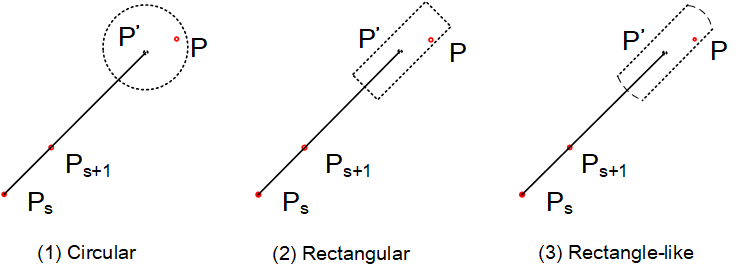
\includegraphics[scale=1.0]{Figures/Fig-Areas.png}\vspace{-1ex}
	%\caption{\small A trajectory is simplified by algorithm \dpa using distance metrics \ped, \sed and \dad, respectively.}
	\vspace{-1ex}
	\caption{\small Trajectory tracking in (1) a floating disc, (2) an infinite beam \cite{Chen:Space,Daescu:metric} and (3) a floating finite beam. Where $P_s$ is the start position of the sub-trajectory and $P'$ is the expected position of the moving object at time $P.t$ whose actually position at that time is $P$.}
	\vspace{-3ex}
	\label{fig:areas}
\end{figure}

\stitle{{Contributions}.}
To the end, we explore ways to track a moving object in disc, infinite beam and finite beam, and design novel one-pass trajectory tracking algorithms that effectively and efficiently run for such areas, respectively. 

\ni (1) We develop a one-pass trajectory tracking algorithm \citt and theoretically prove that it has better effectiveness than \ldrh. Thus, we are able to effectively and efficiently track a moving object in a disc (Section \ref{sec:circle}).
%\citt is more effective than \ldrh, great more efficient and a bit more effective than \grts (Section \ref{sec:circle}).

%\ni (2) We develop a one-pass trajectory tracking algorithm \sitt based on the intersection of sectors that tracks a moving object in a strip area. \sitt is the first algorithm that tracks a moving in a strip area, and is as concise and efficient as \citt (Section \ref{sec:strip}). %, and has a better compression ratio than \citt with a cost of a poorer accuracy.

\ni (2) We provide a convenient way to design new tracking shapes, \ie  infinite and finite beams, and develop novel one-pass trajectory tracking algorithms \sitt and \bitt such that we are able to effectively and efficiently track moving objects in infinite and finite beams (Section \ref{sec:rectangle}). 
%\bitt is the first algorithm that tracks a moving object in a rectangle-like area, and it takes the advantages of both \citt and \sitt (Section \ref{sec:rectangle}). 
%\ie~\sitt based on the intersection of sectors that tracks a moving object in a strip area

\ni (3) Using three real-life trajectory datasets (ServiceCar, GeoLife, Mopsi), we finally conduct an extensive experimental study that compares our methods \citt and \bitt with representative trajectory tracking algorithms \ldrh (the first and the most efficient trajectory tracking algorithm) and \grts (the most effective trajectory tracking algorithm). The experimental results show that \citt and \bitt are both efficient and effective, and are feasible to track a moving object in disc, infinite beam and finite beam (Section \ref{sec-exp}).


\eat{%%%%%%%%%%%%%%%%
\stitle{{Organization}}.
The remainder of the paper is organized as follows:
Section \ref{sec-pre} introduces the basic concepts and the \ldr and \ldrh approaches,
Sections \ref{sec:circle}, \ref{sec:strip} and \ref{sec:rectangle} present three one-pass algorithms that track in circular, strip and rectangle-like areas, respectively,
Section \ref{sec-exp} reports the experimental results of these methods, followed by related works in Section \ref{sec-related} and conclusion in Section \ref{sec-conclusion}.
All proofs are provided in the Appendix.
}%%%%%%%%%%%%%%%%eat


